\documentclass{report}

\input{preamble}
\input{macros}
\input{letterfonts}

\usepackage{tikz}
\usepackage{tikz-3dplot}
\usepackage{amsmath}
\usepackage{pgfplots}
\usepackage{smartdiagram}
\usesmartdiagramlibrary{additions}

\title{\Huge{Lecture Notes}\\Title}
\author{\huge{Giacomo Cappelletto}}
\date{Date}

\begin{document}


\maketitle
\newpage
\pdfbookmark[section]{\contentsname}{toc}
\tableofcontents
\pagebreak

\chapter*{Introduction}

\section{What is this }

\dfn{Definition}{
    \begin{center}
        \textbf{This is some trig function}

        $$z =  sin(x) \cdot cos(y)$$

    \end{center}
    
}

\begin{figure}[h]
\centering
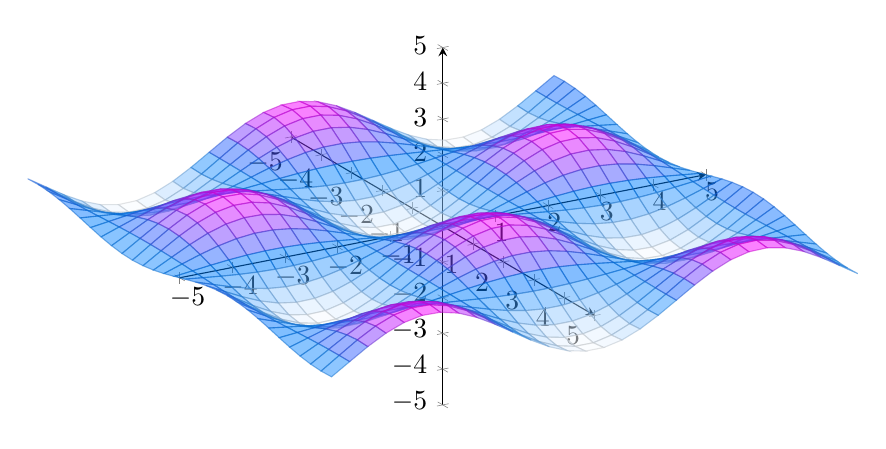
\begin{tikzpicture}
\begin{axis}[
    view={60}{30},
    axis lines = middle,
    xmin=-5, xmax=5,
    ymin=-5, ymax=5,
    zmin=-5, zmax=5,
    xtick={-5,-4,...,5},
    ytick={-5,-4,...,5},
    ztick={-5,-4,...,5},
    width=\textwidth,
    height=0.8\textwidth
]
\addplot3[
    surf,
    domain=-5:5,
    y domain=-5:5,
    samples=30,
    samples y=30,
    z buffer=sort,
    colormap/cool,
    opacity=0.5
]{sin(deg(x)) * cos(deg(y))};
\end{axis}
\end{tikzpicture}
\caption{3D plot of $z = \sin(x) \cdot \cos(y)$}
\end{figure}

\end{document}